% Chapter 2

\chapter{Introduction} % Write in your own chapter title
\label{Chapter2}
\lhead{Chapter 2. \emph{Introduction}} % Write in your own chapter title to set the page header

One of the most important contributions to human health has been vaccination. From the success of Jenner�s and Pasteur�s vaccines against smallpox and chicken cholera, through to the global campaign for the eradication of polio and the widespread immunization against potentially fatal childhood diseases, vaccination has been a vital component of preventative health care. However, the threat of emerging diseases such as avian influenza, as well as current epidemic diseases such as HIV/AIDS, malaria and tuberculosis, has ensured that vaccine development remains a vital component of biomedical research.

One course of vaccination development that has shown recent promise is the identification and utilization of peptide epitopes that stimulate protective immunity. This technique takes advantage of the adaptive immune response to foreign proteins, such as viruses, where pieces of these proteins called epitopes are recognized by the antigen-specific receptors of the immune system (e.g. T-cell receptors, antibodies). Hence, the goal of the vaccine is to safely expose the immune system to pathogenic epitopes to induce an immune response. There are a number of challenges associated with this: identifying what the pathogenic epitopes should be, designing effective delivery of the epitopes when they are found. And increasingly, understanding the complexity of how this works.

The human T-cell lymphotropic virus type 1 (HTLV-I) was the first human retrovirus discovered and its associated diseases: ATL (Adult T-cell leukaemia/lymphoma), HAM/TSP (HTLV-I associated myelopathy/tropical spastic paraparesis) and other chronic inflammatory diseases cause considerable global morbidity and mortality. This chapter gives an overview of the pathogenesis and treatment of the virus and demonstrates the relevancy of my work to understand the basis of an effective immune response towards HTLV-I infection. Hence, a greater understanding of the targets (epitopes) of HTLV-I specific CD8$^+$ T cells may lead to a vaccine against this widespread debilitating virus.

\section{HTLV-I}

\subsection{Virology}

HTLV-I is a type C 
% morphology in negatively-stained E.M.
particle-like onco-retrovirus, and its discovery was first reported in 1980 when a retrovirus was successfully isolated from a T-lymphoblastoid cell line (HUT 102) established from a patient with a cutaneous T-cell lymphoma \citep{Poiesz1980}. This discovery was the first formal proof that human retroviruses exist and suggested their aetiological role in human cancer, a hypothesis that had been proposed decades before \citep{The1993}. The diploid genome consists of 2 identical positive single-stranded RNA molecules each of 9032 bases associated in a complex. It contains the typical retroviral genes of \gene{gag}, \gene{pol} and \gene{env}, and in addition genes encoding regulatory proteins such as \gene{tax} and \gene{rex}.

Gag comprises the structural polypeptides p15 (nucleocapsid), p19 (matrix) and p24 (capsid). Env encodes the envelope protein which is cleaved into the surface glycoprotein gp46 (SU) and the transmembrane protein p21 (TM). Pol encodes the genes for reverse transcriptase, integrase and RNaseH. The rest of the genome contains unique accessory genes in four open reading frames (ORFs) of the pX region of the viral genome, as well as a negative strand product, HTLV-I bZIP-factor (\fref{chapter2/figure2}). The regulatory proteins encoded by pX ORFs III and IV, Tax and Rex, respectively, have been extensively characterized. Tax is a \emph{trans}-acting transcriptional activator. It is of central importance in the dynamics of HTLV-I infection as it is thought to be one of the first to be expressed in the viral life cycle and is a promiscuous transcriptional transactivator. It transactivates both its own LTR and many of those of the infected host cell. It is also central to the host's immune response to the virus as it is the dominant target antigen for the CTL response \citep{Jacobson1990, Kannagi1991, Parker1992, Parker1994, Goon2004}. Rex is an essential shuttle protein required for nuclear export of unspliced and incompletely-spliced viral RNAs \citep{Heger1999}.

Open reading frames I and II are less well known. Both ORFs are alternatively spliced, producing the proteins Rof (p27\superscript{I}) and p12\superscript{I} for ORF I and Tof (p30\superscript{II}) and p13\superscript{II} for ORF II. It was thought that ORFs I and II did not significantly affect viral replication. While the expression of mRNAs for these proteins is well-documented \emph{in vitro} and \emph{ex vivo}, their detection in infected cells has remained elusive. However, a body of evidence suggests that these proteins may be essential for viral persistence. p12\superscript{I} localizes to cellular endomembranes, particularly the ER and expression in virally infected cells could result in decreased expression of MHC class I on the cell surface, thereby protecting infected cells from CTL recognition \citep{Nicot2005}. Recent findings suggest that p30\superscript{II} functions as a post-transcriptional regulator of Tax/Rex mRNA and may also modulate the expression of viral and cellular genes \citep{Nicot2005}. In the presence of Tax, p13\superscript{II} is stabilized and localizes to the nucleus. It has been reported that p13\superscript{II} induces Tax degradation and inhibits its transcriptional activity, thereby decreasing viral replication \citep{Willems2009}.

\begin{figure}[htp]
\centering
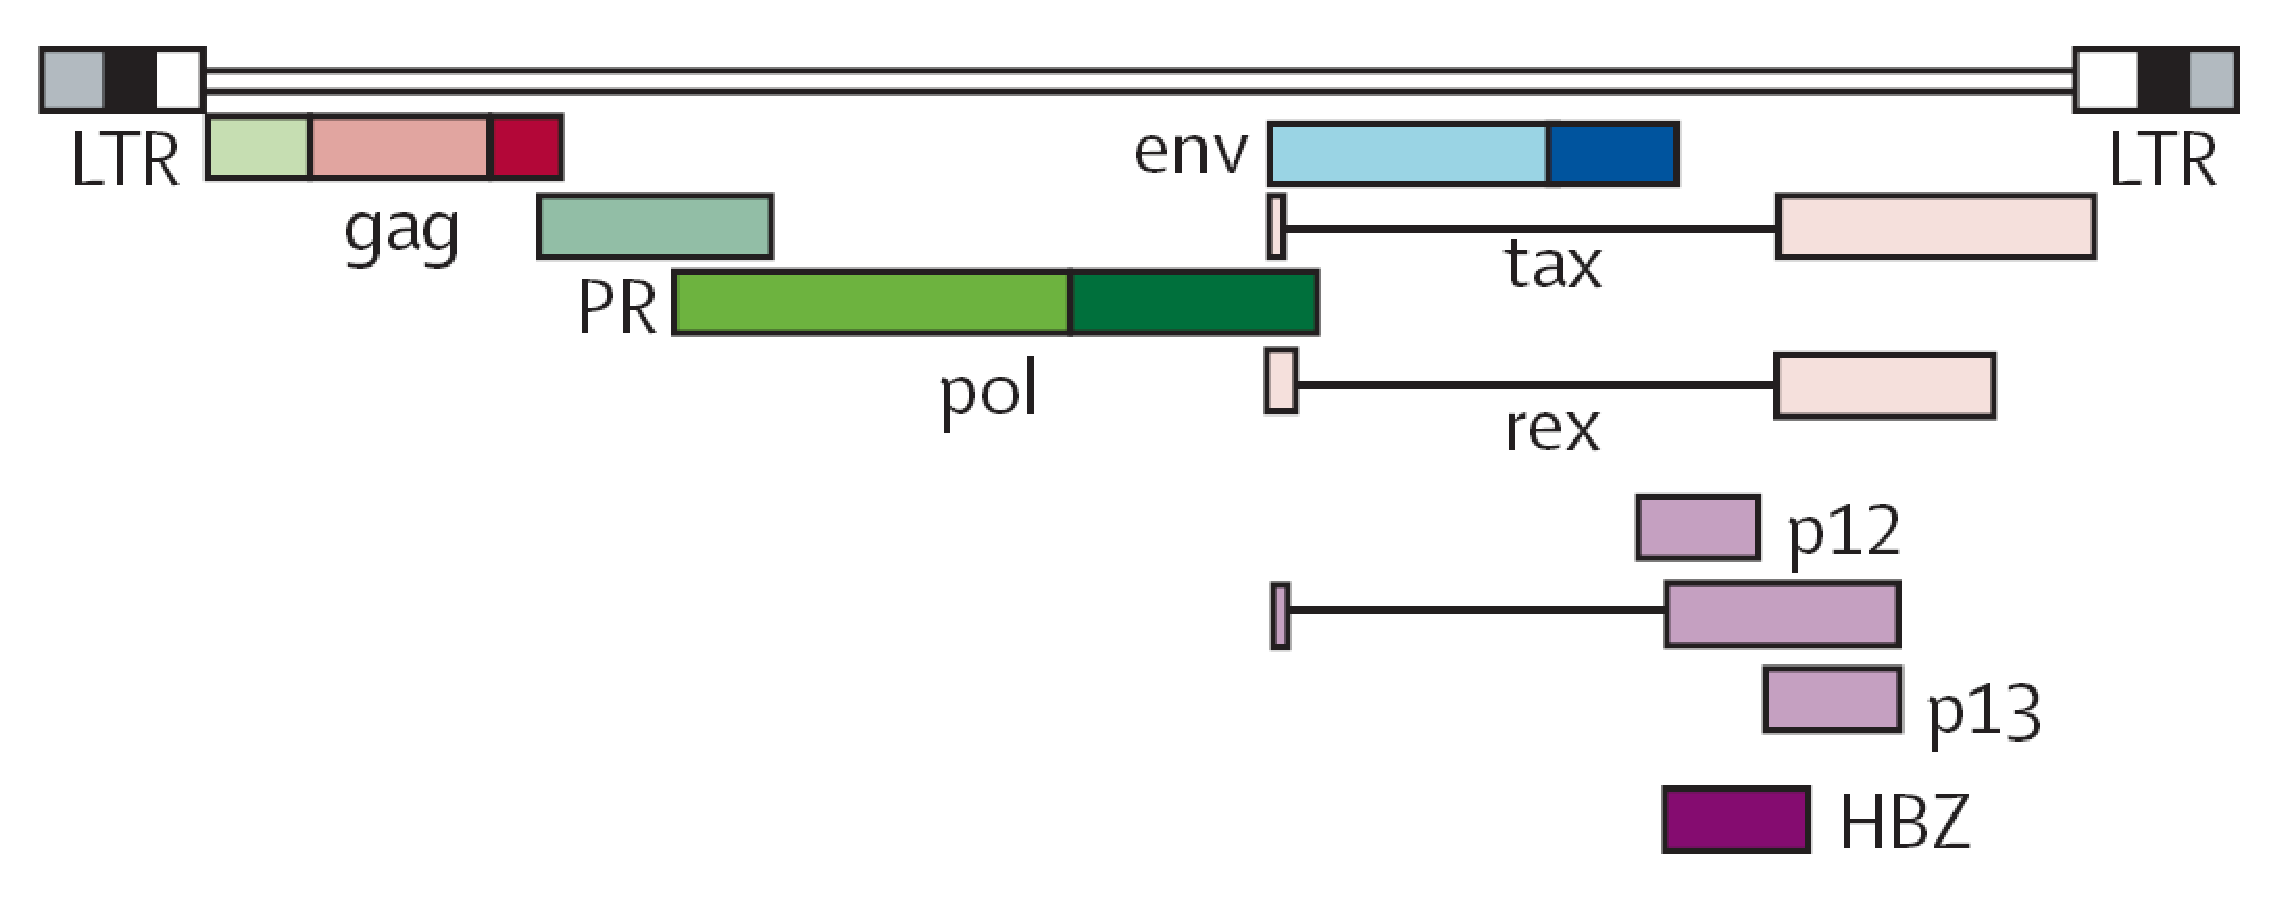
\includegraphics[width=14cm]{./Figures/chapter2/genotype}
\rule{35em}{0.5pt}
\caption[The genomic organisation of HTLV-I]{The genomic organisation of HTLV-I, taken from \citep{Verdonck2007}}
\label{chapter2/figure2}
\end{figure}

It is believed that humans have been exposed to HTLV-I for thousands of years \citep{Novak1999, Gessain2000, Vandamme2000} and HTLV-I viral DNA has been detected in Andean mummies 1,500 years old \citep{Li1999, Sonoda2000}. Even though the virus has been in contact with humans for this amount of time, HTLV-I isolates from Japan, Africa, the Caribbean Basin and the Americas show high sequence conservation (0.5 to 4\%) \citep{Gessain1993}. HTLV-I has been classified into three major lineages known as the Cosmopolitan, Central African and Melanesian groups \citep{Gessain1992, Saksena1992, Gessain1993}. There is further subdivision of the Cosmopolitan group into four subgroups based on LTR sequencing; these are the (A) Transcontinental, (B) Japanese, (C) West African and (D) North African \citep{Gasmi1994, Miura1994}. Generally, a single viral genotype is found in any one location but in Kagoshima, Southern Japan, both Cosmopolitan A (Transcontinental) and B (Japanese) coexist because of its location between Honshu Island (Cosmopolitan B) and Okinawa (Cosmopolitan A) \citep{Vidal1994a, Furukawa2000}.

The virus infects T-cells, with CD4$^+$ and CD45RO$^+$ T-lymphocytes being the main targets for infection \citep{Hanon2000a, Richardson1990}. CD8$^+$ T-cells have also been shown to act as as reservoir for the virus \emph{in vivo} \citep{Nagai2001, Hanon2000b}. HTLV-I can spread directly between lymphocytes across a specialized, virus-induced cell-cell contact - a `viral synapse' \citep{Bangham2003}. The cellular receptor for HTLV-I has not been identified, despite intensive efforts over many years. However, its presence has been demonstrated by virus-induced cell fusion experiments, leading to syncytium formation \citep{Hoshino1983, Nagy1983}. It has been mapped to chromosome 17 (17q region) \citep{Sommerfelt1988} but it is possible that this site encodes not the putative receptor but just an essential cofactor. 

\subsection{Epidemiology}

\begin{figure}[htp]
\centering
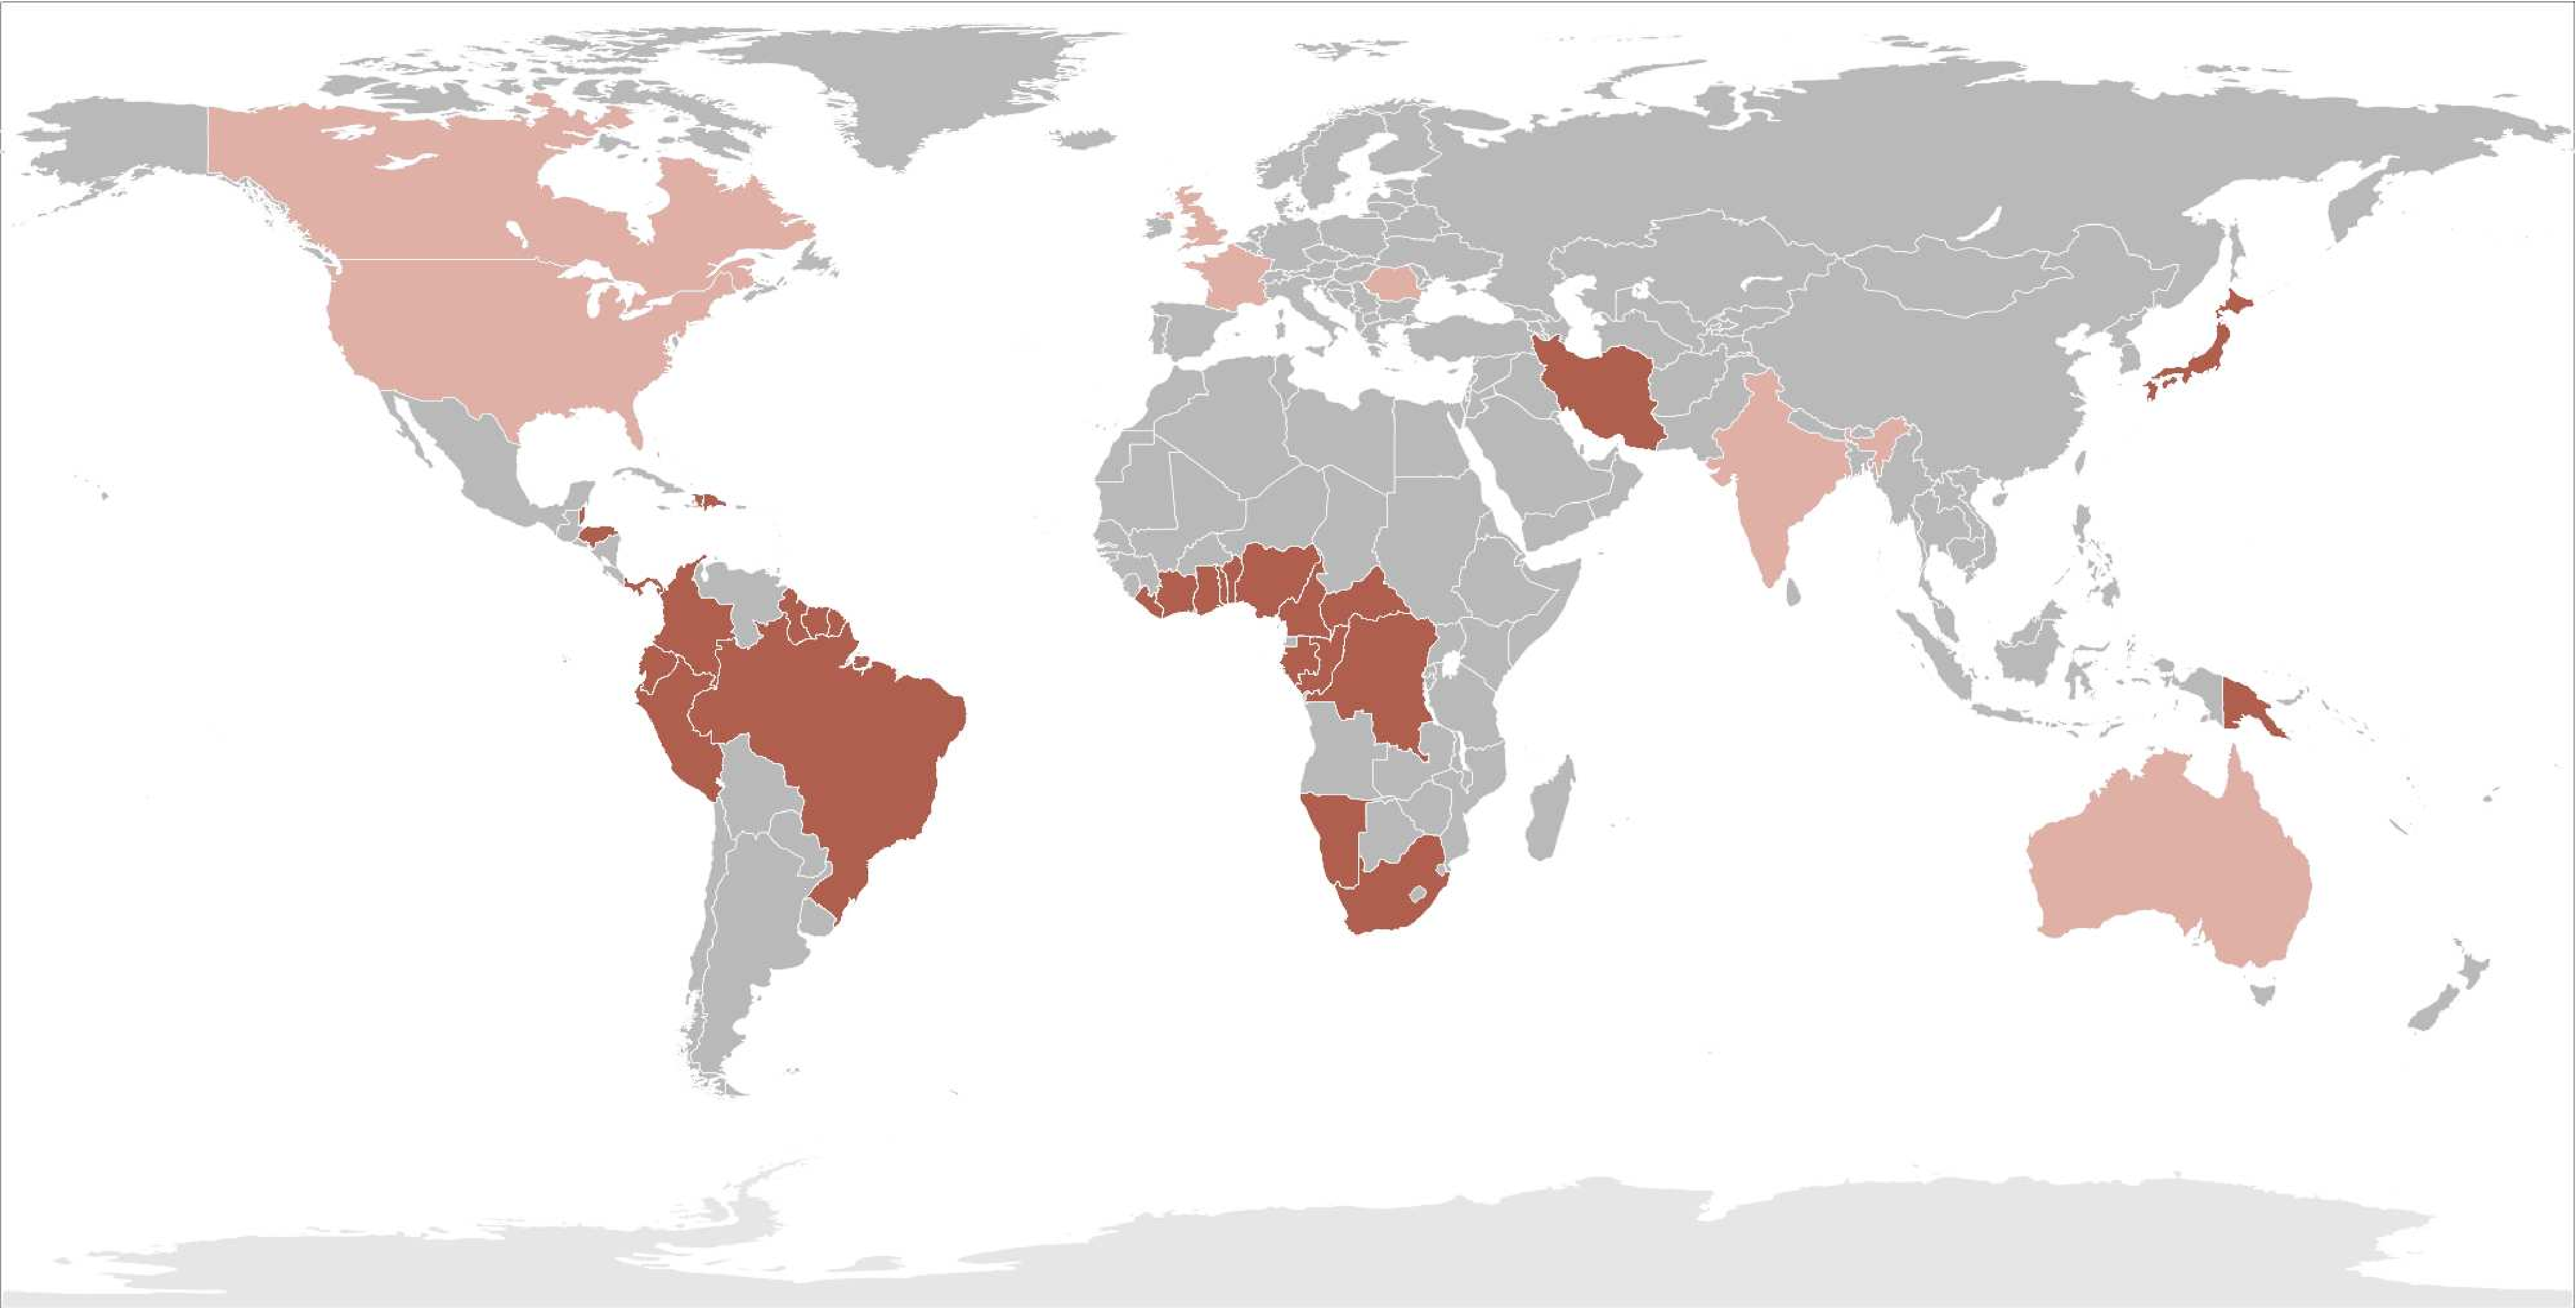
\includegraphics[width=14cm]{./Figures/chapter2/distribution}
\rule{35em}{0.5pt}
\caption[The global distribution of HTLV-I]{Countries with endemic HTLV-I, defined as prevalence between 1 and 5\% in some populations, are shown in dark red. Countries with reports of low prevalence (less than 1\% in some groups), due mainly to immigration from endemic areas, are shown in light red. It should be noted that HTLV-I endemic areas do not correspond exactly to the country boundaries shown in the map. For example in Brazil, Japan and Iran, HTLV-I is limited to residents of certain areas of each country. Data is from \citep{Proietti2005}.}
\label{chapter2/figure1}
\end{figure}

The virus is endemic to a number of geographically distinct regions across the world (\fref{chapter2/figure1}). In the Caribbean, 3-4\% of the population are seropositive for HTLV-I, in Africa the virus is detectable along an increasing gradient from north to equatorial Africa and in Japan, several regions have high incidences of seropositive individuals \citep{Edlich2000}. It can also be found in northern Iran, southern India and the aboriginal peoples of northern Australia. Other populations include immigrants from these endemic areas, as well as sporadic cases of HTLV-I among white Europeans with no identifiable risk factors. Overall, it is estimated to infect between 10 and 20 million people worldwide \citep{The1993}. It is a chronic infection which remains asymptomatic in the majority of cases. There is a maximum seroprevalance of 35\% in Okinawa, Japan \citep{Hinuma1982}.

The principal modes of transmission are transfer of infected CD4$^+$ lymphocytes from mother to child in breast milk, sexual transmission (especially from infected men to women via semen) and via inoculation/transfusion of infected blood. Cell-free blood products have a negligible risk because of the paucity of free virus particles present in plasma. Infection in endemic regions occurs mainly through breast-feeding, via the transfer of infected lymphocytes in the milk \citep{Hino1985}. However, infection can occur during the peri-natal period \citep{Hino1987} and transplacental transmission has been documented but is not thought to be common \citep{Komuro1983}. Male to female transmission is roughly 4 times higher than the converse \citep{Stuver1993} and the risk of infection is increased in the presence of genital ulceration, high proviral loads and high antibody titres \citep{Murphy1989, Kaplan1996}. The probability of seroconversion following transfusion of infected blood products is 50-60\% with a median time to conversion of 51 days \citep{Okochi1984, Manns1992}. Screening transfusion blood for HTLV-I is now routine in Brazil, Japan, the UK and the USA. There is an increasing prevalence of HTLV-I among intravanous drug users in both Europe and the USA \citep{The1993}.

\section{HTLV-I Associated Diseases}

Most HTLV-I-infected people remain healthy, but between 1-2\% will develop HAM/TSP, another 2-3\% develop ATL and a small number develop other less well defined inflammatory disorders. The factors deciding these outcomes are not fully understood but they are two distinct pathologies and the pathogenesis of the two appear to be very different. It has been thought that the occurrence of the two syndromes in the same person is not seen any more frequently than would be expected by chance. However, a high frequency of co-presentation of HAM/TSP and ATL has recently been reported in Bahia, Brazil \citep{Willems2009}.

\subsection{HTLV-I Associated Myelopathy/\\Tropical Spastic Paraparesis (HAM/TSP)}\label{chapter2/HAM/TSP}

The first descriptions of a myelopathy of unknown origin in tropical areas go back to the 19\superscript{th} century \citep{Strachan1888}. The association with HTLV-I was recognized independently in the Caribbean (as TSP) and in Japan (as HAM) in 1985-1986 \citep{Gessain1985, Osame1986}. The lifetime risk for developing HAM/TSP is between 2-7\%, except for Japan where it is estimated to be 0.25\% \citep{Kaplan1990, Taylor2000}.

\subsubsection{Pathology}\label{chapter2/path}

The main pathological feature of HAM/TSP is a chronic inflammation of the white and grey matter of the spinal cord. Mononuclear cells, mainly T cells, cause 
% perivascular cuffing - accumulation of lymphocytes / parenchyma
perivascular cuffing and infiltrate the parenchyma \citep{Verdonck2007}. The damage is concentrated in the white matter of the lower thoracic spinal cord, which causes the spastic paraparesis in the lower limbs \citep{Aye2000}. There is a possibility that the lesions in the central nervous system could be the consequence of a genuine anti-HTLV-I reaction. This is based on the observations that HAM/TSP patients have a higher proviral load, a higher production of proinflammatory cytokines in response to viral peptides (such as IFN-$\gamma$ and TNF$\alpha$) and a higher frequency of HTLV-I specific CD8$^+$ T-cells compared to asymptomatic carriers \citep{Olindo2005, Sakai2001, Goon2003, Montanheiro2005}. Polymorphism in the TNF$\alpha$ promoter and the chemokine gene SDF-1$\alpha$ have also been shown to influence the risk of HAM/TSP \citep{Vine2002}. Other evidence of an immunopathological reaction in the central nervous system is the observation of infected T-cells within the spinal cord lesions and the accumulation of Tax-specific CD8$^+$ T-cells in the cerebrospinal fluid \citep{Kubota2002, Muraro2003}. There is also a possibility that cross-reactivity between HTLV-I antigens and tissue antigens could be involved in the pathogenesis. This is based on a contentious finding that patients with HAM/TSP appear to develop antibodies to human neurons but not to systemic organs \citep{Levin2002}. Additionally, auto-antibodies against other nuclear and perinuclear human brain proteins cross-reacting with different HTLV-I epitopes have been found in the serum of HAM/TSP patients \citep{Garcia-Vallejo2005}. However, since inflammatory T-cells, rather than antibodies, seem to cause the tissue damage, autoreactivity at the level of the T-cell receptor may be more likely.

\subsubsection{Presentation}

The commonest presenting features in descending order are gait disturbance ($\sim2/3$ cases), urinary dysfunction ($>1/3$ cases), then numbness of the lower legs, constipation, lumbar back pain and hand tremors. The lower limbs are usually affected to a much greater degree than the upper limbs. The spasticity and associated upper motor signs can be very severe. Low back pain or ache is very common and affects most at some time during the course of the disease. The spectrum of disease progression is very variable, ranging from minimal gait disturbance maintained over the patient�s lifetime
to severe, very rapid progression and even death (rare). In one study cohort from Columbia, after a mean period of 14.4 years (range of 1 - 30 years), 34\% could walk unaided, 40\% required a walking aid, and 26\% required a wheelchair (otherwise bed-bound) \citep{Roman1988}.

\subsubsection{Treatment}

Therapies targeting the immune response have been considered for the treatment of HAM/TSP. Corticosteroids have been shown to be of some benefit \citep{Nakagawa1996} and interferon-$\beta$1a reduced HTLV-I mRNA load. However, the proviral load remained unchanged and there was only a slight improvement in motor function \citep{Osame1990} The combination of two nucleoside analogues (zidovudine and lamivudine) has been evaluated in a randomised, double-blind, placebo-controlled study including 16 HAM/TSP patients. After up to 12 months of follow-up, there were no significant changes in proviral load and no clinical improvement was observed \citep{Taylor2006}. Long term treatment studies have been formulated with valproic acid (VPA). VPA is a lysine deacetylase inhibitor and is postulated to work by activating viral gene expression and exposing virus-infected cells to the immune system, thus reducing proviral load. It has been shown to be safe but does not seem to alleviate the conditions of HAM/TSP \citep{Willems2009}. Additional strategies that have been proposed include minocycline (an antibiotic that inhibits monocyte/macrophage activation), humanized mik$\beta$1 (a monoclonal antibody against CD122, the $\beta$ subunit shared by IL2 and IL15) and the immunosuppressant cisclosporin \citep{Willems2009}.

\subsection{Adult T-cell Leukaemia/Lymphoma (ATL)}

ATL was first described in the 1970s when the observation of haematological malignancies did not fit previous pattern descriptions \citep{Yoshida2001}. It is a malignancy of CD4$^+$ post-thymic T-cells in which the HTLV-I provirus is integrated.

\subsubsection{Pathology}

The regulatory protein Tax induces abnormal growth of infected T-cells through several pathways \citep{Yoshida2001}. Tax promotes the transcription of its own proviral genome, but it also promotes transcription of cellular genes, including cytokine (e.g.~interleukin-2), cytokine receptor (interleukin-2Ra), and anti-apoptotic genes. By binding to other protein complexes, Tax represses the transcription of genes that are important in negative control of the cell cycle, in activation of apoptosis, and in DNA repair. Tax also binds and inhibits proteins directly involved in tumour suppression and DNA repair. Finally, Tax causes cells to bypass normal cell-cycle checkpoints \citep{Yoshida2001}. The net effect of all these activities of Tax is that T cells are rushed into and through the mitotic phase without checking for chromosomal abnormalities. Genetic damage that would normally be repaired accumulates and apoptotic cell death does not occur even in cells with severely damaged DNA. In these circumstances, T cells can accumulate DNA mutations, resulting in transformation and monoclonal outgrowth of a truly malignant cell. In addition to these genetic changes, epigenetic changes such as DNA methylation may have an important role in leukaemogenesis \citep{Taylor2005}.

\subsubsection{Presentation}

There are several types of HTLV-I induced ATL: acute, lymphotamous, chronic and smouldering \citep{Shimoyama1991}. Amost all patients with ATL present with lymphadenopathy (enlargement of the lymph nodes) and/or splenomegaly (enlargement of the spleen). ATL can also affect the lungs, gastrointestinal tract, and central nervous system; involvement of other organs is uncommon \citep{Shimoyama1991}. Hypercalcaemia is an important complication: it occurs in up to 70\% of patients and is often accompanied by lytic bone lesions. ATL patients are immunosuppressed and opportunistic infections, such as \emph{Pneumocystis jirovecii} pneumonia, cryptococcus meningitis, and disseminated herpes zoster are, therefore, frequent \citep{Roudier1997}. Liver dysfunction is another complication. The diagnosis of ATL is usually based on morphological analysis. Flower cells (i.e.~pleomorphic, atypical lymphoid cells with basophilic cytoplasm and convoluted nuclei) are indicators of acute or lymphoma-type ATL. This must be confirmed by clonal integration of HTLV-I provirus in the host genome.

\subsubsection{Treatment}

Acute ATL is very aggressive and highly refractory to treatment. Strategies that show an improvement over conventional chemotherapy in the treatment of ATL include Interferon-$\alpha$ with zidovudine, intensive chemotherapy and allogenic haematopoietic stem cell transplantation \citep{Taylor2005}. In fact, it is essential not to provide general chemotherapy (CHOP) to first line presenting ATL patients because this treatment selects for a tumor clone with mutated p53 \citep{Tsukasaki2009}. Nevertheless, the median survival of patients with acute, lymphomatous, and progressing chronic ATL remains low: less than 1 year in most reports \citep{Taylor2005}. Further improvements could include bortezomib (a proteasome inhibitor), anti-CD52 antibody, proapoptotic agents and consolidation with arsenic and IFN$\alpha$ \citep{Willems2009}. 

\subsection{Other Conditions Associated with HTLV-I}

HTLV-I has been associated with other inflammatory syndromes. In a Japanese cross-sectional study and a US cohort study, the prevalence and the incidence of arthritis were found to be higher among HTLV-I-infected patients than among uninfected individuals \citep{Eguchi1996,Murphy2004}. Tax transgenic mice have also developed an arthritis that is pathologically similar to human rheumatoid arthritis \citep{Iwakura1991,Yakova2005}.Tax has been shown to stimulate the proliferation of synovial cells in vitro \citep{Aono1998}. Hence, Tax, released by HTLV-I-infected cells in vivo, could have a part in the pathogenesis of arthropathy.

Reports from Japan have shown that HTLV-I infection is more frequent in patients with uveitis of unknown origin than in the general population \citep{Mochizuki1992}.The prognosis of HTLV-I-associated uveitis is good: spontaneously, the disease resolves within weeks and recovery is even faster with topical or systemic corticosteroid treatment. However, more than 90\% of cases recur within 3 years; the mean interval between episodes is 16 months \citep{Nakao1999}.

\emph{Strongyloides stercoralis} is an intestinal nematode of tropical regions that can replicate within the human host, an unusual characteristic among helminths. HTLV-I infection is associated with increased susceptibility to \emph{S. stercoralis} infection and a weak Th2 response is characteristic of this co-infection. As a result, the rate of parasite killing decreases and the rate of autoinfection increases \citep{Carvalho2004}. In rare cases this can result in the fatal Strongyloides hyperinfection syndrome \citep{Marcos2008}.

\section{Pathogenesis of HTLV-I}\label{chapter2/pathogenesis}

\subsection{Background}

1-2\% of HTLV-I infected subjects develop HAM/TSP and 2-3\% develop ATL. The factors deciding these outcomes of infection are not understood.

\subsection{Genotype}

Compared with HIV, HTLV-I is relatively stable in terms of sequence variation and mutation rate. However, the effect of mutation on the pathology of HTLV-I is still considered a possible variant in disease outcome. As a result, HTLV-I has been the subject of a range of studies looking at mutation and variability and how this affects the immune response to the virus. The majority of these studies have focused on \gene{tax}, as it is a dominant target for the CD8$^+$ immune response \citep{Goon2004}. Furukawa \emph{et al.} \citep{Furukawa2000} found phylogenetic subgroups in the \gene{tax} gene, one of which was associated with an increased risk of HAM/TSP. This result followed on from a number of studies from Niewiesk \emph{et al.} that focused on Tax expression. 

Initially, Niewiesk \emph{et al.} found that general \gene{tax} sequence variability (and not the presence of a specific sequence) was significantly greater in healthy seropositive individuals, compared to those presenting HAM/TSP \citep{Niewiesk1994}. This was followed by results showing that amino acid substitutions occurring in known Tax epitopes abolished T cell recognition. These substitutions were also associated with the allele \gene{HLA-A2} and reduced the transactivation function of Tax \citep{Niewiesk1995}. However, it was then found that this distinction in the mutation rate of \gene{tax} between healthy individuals and those with HAM/TSP could only be seen with proviral \gene{tax} sequences, but not with cDNA \citep{Niewiesk1996}. Kubota \emph{et al.} looked at synonymous and nonsymonymous \gene{tax} mutations in \gene{HLA-A*02} HAM/TSP patients to detect positive selection pressures \cite{Kubota2007}. They found pressures on three of six CTL epitopes tested, suggesting that CTLs eliminate infected cells \emph{in vivo} and also demonstrating that variant viruses do not accumulate. Once again, this reinforced the observation that Tax is functionally constrained in terms of mutations. Although research on Tax has predominated, some work on other proteins has also been completed. Furukawa \emph{et al.} showed that sequence variation in p12 may be associated with different outcomes to HTLV-I infection \citep{furukawa2004}. The Rex protein was also examined and shown to have strong functional constraints on amino acid variation \citep{Smith1997}. 

\subsection{The CTL Response to HTLV-I}\label{chapter2/CTLResponse}

The CTL response plays a central role in deciding the outcome of viral infections. It has been shown through evidence accrued from host and viral genetics, gene expression microarrays and assays of T-cell phenotype and function that individual differences in the efficiency of the virus-specific CTL response strongly determine the outcome of infection with the human retroviruses HTLV-I and HIV-I. From this evidence, it is now believed that differences in the anti-viral CTL efficiency at the single-cell level are responsible for variation in the efficacy of the host response to viruses.

Perhaps the strongest evidence that the CTL response is instrumental in controlling HTLV-I infection comes from the association of certain MHC class I alleles and protection from disease. Studies of HTLV-I genotype show significant associations between class I alleles (HLA-A*02 and HLA-Cw*08) and a reduced proviral load, which would implicate the CTL response as a positive factor \cite{Jeffery1999, Jeffery2000}. The hypothesis that extends from these results is that HLA-A*02 and HLA-Cw*08 restricted CTLs are more efficient at killing HTLV-I infected cells. Conversely, HLA-B*54 restricted CTLs, which have been associated with increased proviral load~\cite{Jeffery1999}, would produce a less efficient response.

The frequency of virus-specific CTL has been used to demonstrate the efficiency of the CTL response in HTLV-I infection with different conclusions. There is evidence that the frequency of HTLV-I-specific CD8$^+$ T cells differs little among patients with widely differing proviral load \citep{Parker1994}. However it has also been reported that HTLV-I-specific CTL frequency was positively correlated with proviral load \citep{Kubota2000}. These contradictory results demonstrate the difficulty of using CTL frequency as a marker of viral control in a chronic infection: since CTL proliferate in response to antigen, the frequency of CTL is both a cause and an effect of the viral load. Hence, a more effective metric of CTL efficiency is a measurement variable that accurately reflects an efficient CTL response.

CD8$^+$ cell attributes such as T-cell receptor avidity, specificity, and cell maturation state may all affect the ability of CD8$^+$ cells to control a viral infection. However, Asquith \emph{et al.} devised a combined measure by measuring the rate at which naturally, endogenously infected cells were cleared by autologous CD8$^+$ cells \emph{ex vivo} \citep{Asquith2005a}. This antiviral efficacy can be summarised by \eref{chapter2/equation1}: 

\begin{equation}
\frac{dy}{dt} = c - \epsilon y z
\label{chapter2/equation1}
\end{equation}

where $y$ is the proportion of CD4$^+$ cells expressing Tax, $c$ is the rate of increase of Tax expression, $\epsilon$ is the CD8$^+$ cell-mediated antiviral efficacy and $z$ the proportion of lymphocytes that are CD8$^+$. This approach yielded the conclusions that there was a significant negative correlation between the per-CD8$^+$ cell lysis rate and the proviral load, in both ACs and HAM/TSP patients. Also, the percentage of between-individual variation observed in the proviral load that was attributable to variation in the lysis rate parameter was about 35\% \citep{Asquith2005a}. From this data, it was predicted that CTL lysis would reduce the life expectancy of a virus-expressing target cell from the normal 30 days (for a memory phenotype, CD4$^+$CD45RO$^+$ T cell) to between 1 and 10 days. This was confirmed by measurement of infected T-cell turnover rate \emph{in vivo} by the metabolic labeling of lymphocytes with deuterated glucose \citep{Asquith2007a}.

The functional avidity is the concentration of antigen that is required to elicit the half-maximal effector response (usually
cytokine) in CD8$^+$ T cells. It has been widely used as a marker of the responsiveness or sensitivity of CTL to cognate antigen. In HTLV-1 infection, Kattan \emph{et al.} \citep{Kattan2009} found that avidity was correlated with per-CD8$^+$ lytic activity, measured by the CD8-dependent elimination of Tax$^+$ cells. The use of CD107a staining of CD8$^+$ T cells as a marker of the recent degranulation activity of HTLV-I-specific CD8$^+$ T cells has also shown differences between HAM/TSP patients and ACs; HAM/TSP patients produced a greater frequency of specific CD8$^+$ T cells but less CD107a staining per cell than ACs \citep{Sabouri2008}.

Taken together, this data emphasizes the role of CTL in HTLV-I control. It is clear that the HTLV-I-specific CTL response plays a critical role in limiting the replication of HTLV-I, the proviral load, and the risk of HAM/TSP. However, any understanding of the role of the CTL response in HTLV-I infection must acknowledge the seemingly detrimental effects of this response to the host (\sref{chapter2/path}).  

\subsection{The Antibody Response to HTLV-I}

Anti-Gag antibodies are the first specific antibodies to appear in response to the infection in the first 2-3 months. Anti-Env antibodies can then be detected, along with anti-Tax antibodies in 50\% of infected people \citep{Manns1992, Mueller1997}. Anti-HTLV-I antibody titres correlate with the provirus load and can be extremely high. It is currently unknown whether these antibodies play a part in protection against HTLV-I infection, against disease or are involved in the pathogenesis of disease.

Levin \emph{et al.} \citep{Levin2002} have described a putative autoantigen; neuronal heterogeneous nuclear ribonuclear protein-A1 (hn-RNP-A1), which stained brightly with IgG from HAM/TSP patients and not ACs. These IgG were also found to cross-react with HTLV-I Tax protein and stained human Betz cells specifically. Furthermore, the authors infused these antibodies onto rat brains and showed inhibition of neuronal activity. Thus, they concluded that HAM/TSP is an autoimmune disease, with molecular mimicry between an HTLV-I antigen and a self one causing the generation of cross-reacting antibodies and subsequent neurological disease.

\subsection{Other Immune Responses to HTLV-I}\label{chapter2/OtherImmune}

T\subscript{reg} cells are defined as CD4$^+$ T cells that inhibit immunopathology or autoimmune disease \emph{in vivo} \citep{O'Garra2004a}. The subset that has been studied with respect to HTLV-I is characterized by the expression of the glycoproteins CD4 and CD25, as well as the transcription factor Foxp3 \citep{O'Garra2004a}. Their role in HTLV-I infection is not yet fully understood but different T\subscript{reg} responses have been associated with both ATL and HAM/TSP. In terms of HAM/TSP, a number of studies have found that in T\subscript{reg} cells infected with the virus, both mRNA and protein expression of Foxp3 were lower in HAM/TSP patients compared to healthy carriers \citep{Yamano2005, Oh2006}. This has lead to the hypothesis that defects in T\subscript{reg} expression as a result of viral infection could cause the chronic inflammatory response characteristic of HAM/TSP \citep{Fujinami2005}. However, this conclusion remains very uncertain because HTLV-I strongly induces expression of CD25 (a marker of T\subscript{reg} cells) and it is therefore inappropriate to use CD25$^+$ as part of the definition of T\subscript{reg} cells in HTLV-I infection (C. Bangham, pers. comm.).

In terms of ATL, several studies have shown the expression of Foxp3 in the tumour cells of a subset of patients with ATL \citep{Yano2007}. Yano \emph{et al.} demonstrated these cells continue to act as regulatory T cells and that their proliferation may be the cause of the severely immunocompromised state of ATL patients \citep{Yano2007}. 

The natural killer (NK) cell response to HTLV-I has received less attention, partly because of the difficulty in identifying NK cells in terms of their surface markers and the existence of NK cell subsets \citep{Bangham2005}. However, an association has been found between the low frequency of CD3$^+$ NK cells and patients with HAM/TSP \citep{Saito2003, Yu1991, Fujihara1991}, suggesting a role for this subset of NK cells in disease progression. Other data on lymphocyte gene expression also indicated that high levels of expression of certain genes involved in NK cell-mediated lysis were associated with low proviral load of HTLV-I \citep{Vine2004}. This would suggest that, along with CD8$^+$ CTLs, NK cells are part of the cytolytic lymphocytes that reduce HTLV-I proviral load.

The CD4$^+$ (helper) T cell response has been difficult to study as Tax in infected CD4$^+$ T cells produces effects (IFN$\gamma$ production, T-cell proliferation), which are also the basis of CD4$^+$ T cell response assays \citep{Bangham2005}. Hence, the presence of HTLV-I would interfere with any analysis on CD4$^+$ T cell response. However, using a modified assay \citep{Goon2002}, it has been demonstrated that the response is predominantly IFN$\gamma$-producing cells. Also the frequency of IFN$\gamma$ producing CD4$^+$ T cells was between 10 and 25 times greater in HAM/TSP patients compared with asymptomatic carriers \citep{Goon2003}. From this information, it is likely that these cells contribute to the chronic inflammatory response seen in HAM/TSP. 

\section{Epitope Prediction}\label{Introduction/Prediction}

As mentioned in \cref{Chapter1}, \sref{chapter1/EpPred} it was necessary to use epitope prediction software to predict the HTLV-I peptides that bind to different MHC class I alleles. This type of prediction software uses a range of mathematical methods to recognize the small number of pathogenic peptides that can bind to MHC class I and hence elicit a CTL immune response.

Of the large number of peptides that can be derived from a pathogen only a small minority, approximately 1 in 2,000, elicits a CTL response \citep{Yewdell1999}. This limitation in the number of peptides that are immunogenic is conferred by three main constraints: the requirement for peptide cleavage and transport, the requirement for MHC-peptide binding and the requirement for CTL recognition. By far the most stringent of these is the requirement for MHC-peptide binding, because only 1 in 200 peptides binds a specific MHC molecule with sufficient affinity to elicit an immune response \citep{Yewdell1999}. Further selection is largely due to the limitations of peptide processing and transport. In these processes, individual peptides are produced from the precursor polypeptides by proteasomal cleavage of the polypeptide, which can be followed by N-terminal trimming by other peptidases. This is followed by the transport of the peptides from the cytosol to the endoplasmic reticulum, mediated by the TAP complex. Further N-terminal trimming may occur before the peptide binds to the MHC molecule. The requirements of processing and transport eliminate approximately 80\% of potential epitopes \citep{Yewdell1999}. Finally, T cell specificity, i.e. the requirement for T cell receptor binding of the MHC-peptide complex, further halves the number of presented peptides that elicit a response. The probability of each of these steps is determined by the polypeptide sequence, amongst other factors \citep{larsen2005}.

The identification of T cell epitopes is of vital importance in the design of vaccines and understanding of the immune system \citep{bui2006, sette2005, sette2007, sathiamurthy2005}. However, given the scarcity of epitopes, experimentally screening all possible peptides for each MHC allele (e.g. by IFN$\gamma$ ELISpot) is time consuming, expensive and inefficient. One way to improve the efficiency of the identification process is to first use theoretical algorithms to predict which peptides are more likely to be epitopes and then experimentally screen this much smaller, selected list of peptides. This method is widely used \citep{snyder2004, tscharke2005, drexler2003, oseroff2005, pasquetto2005} and has been applied in a number of studies to identify potential vaccines \citep{wang2007a, thorn2007}. The use of theoretical methods to "pre-screen" peptides is of particular importance in the case of emerging infections such as avian influenza \citep{wang2007} where rapid vaccine development would be vital. This approach also underpins a large bio-preparedness initiative coordinated by the Large-Scale Antibody and T Cell Epitope Discovery Program \citep{sette2005}, which intends to foster development of immune-based therapeutics for emerging and reemerging pathogens including potential bioterrorism agents. More generally, epitope prediction algorithms are being increasingly used to understand the CTL response. For example, in the case of HIV-I infection, algorithms have been used to confirm which epitope mutations are likely to confer escape from a CTL response \citep{brumme2007} and to understand why some MHC class I alleles are associated with slow rates of disease progression \citep{borghans2007}.

A range of computational algorithms have been developed to predict CTL epitopes in pathogen protein sequences. Since the most selective requirement for a peptide to be immunogenic is the ability of the peptide to bind to the MHC molecule, most prediction methods focus on this stage of the pathway. As a general rule, information gained from experimental binding assays is used to train the algorithm until it is efficient at predicting novel MHC-peptide complexes. The algorithms that are used vary in complexity and accuracy. Some can be trained to recognize peptide motifs that are required for binding to a particular MHC molecule \citep{rammensee1999}, others use a weight-matrix method to identify amino acids that occur at a higher-than-expected frequency at specific epitope positions \citep{nielsen2004, bui2005, peters2005a}. However, the most accurate methods available use logistic regression \citep{heckerman2007} and, more generally, artificial neural networks \citep{larsen2005, tenzer2005}.

Artificial neural networks (ANNs) take into account, in addition to the identity of each amino acid residue, the interactions between adjacent amino acids in a potential epitope. In summary, an ANN for a particular MHC molecule is trained to recognize associated inputs (a peptide sequence) and outputs (the binding affinity for that sequence with the MHC molecule) \citep{buus2003}. Once an ANN is trained for a particular molecule, it can predict the binding affinity of novel peptide sequences.

NetCTL \citep{larsen2005} and NetMHC \citep{buus2003, nielsen2003, nielsen2004} are two of the most accurate prediction methods currently available \citep{peters2005}. NetMHC uses ANNs for a number of alleles to predict MHC molecule-peptide binding affinities. NetCTL, as well as using the same ANNs to predict MHC-peptide binding, also utilizes information about the proteasomal cleavage of the input peptide sequence, and its ability to bind to TAP. NetCTL or NetMHC will predict a score (either integrated or simply a binding affinity, respectively) for every overlapping nanomer peptide sequence in an input sequence to each MHC molecule for which the method has an ANN. Henceforth, we refer to the trained prediction algorithm for each MHC class I allele as an "allelic predictor".